\newpage
\section{Conclusions}
To conclude, the proposed gripper represents a good compromise between functionality, adaptability and manufacturing simplicity. The final solution satisfies the main requirements defined at the beginning of the project, allowing the component to be grasped from the safe lower cylindrical surface while avoiding the restricted areas.

The two-claw under-actuated quadrilateral architecture, together with the replaceable rubber attachments and the simplified mechanical structure, supports a stable pick-up, easy maintenance and a feasible assembly process. For these reasons, the design can be considered suitable for the required task.

Finally, the final CAD test confirms that the gripper can close correctly, as seen in the test below, conducted with the component with the largest diameter. The claws remain aligned with the safe contact areas and avoid interference with the flanges, validating the design approach used.

\begin{figure}[H]
	\centering
	\begin{minipage}{0.45\textwidth}
		\centering
		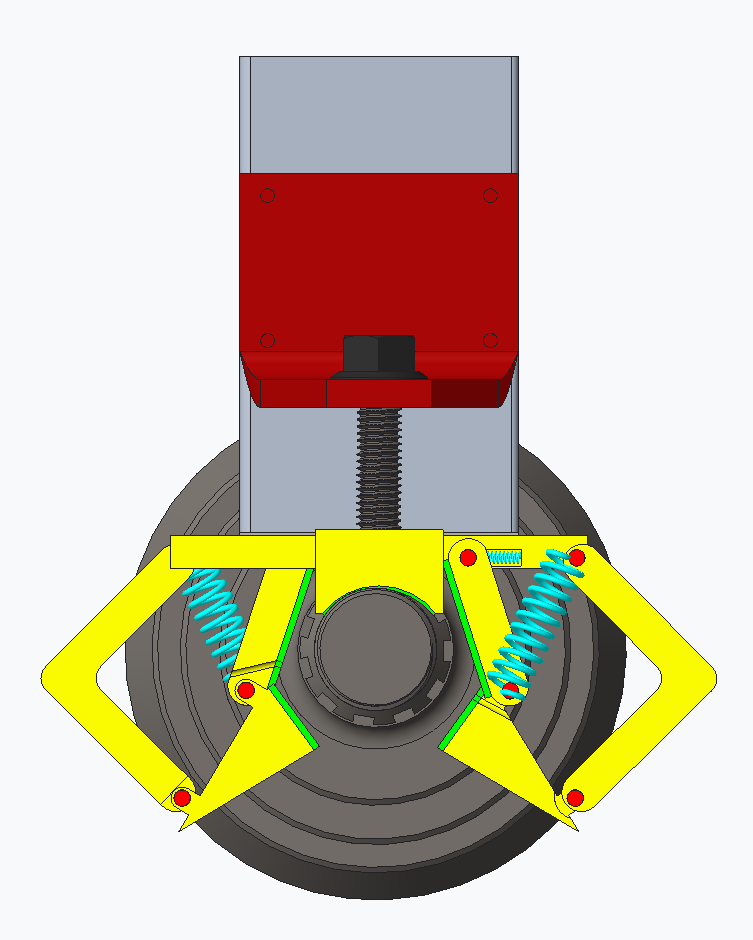
\includegraphics[width=\textwidth]{Immagini/mechanism front.png}
		\caption*{Test start:\\ the gripper has enough tolerance prior to motion}
	\end{minipage}
	\hfill
	\begin{minipage}{0.45\textwidth}
		\centering
		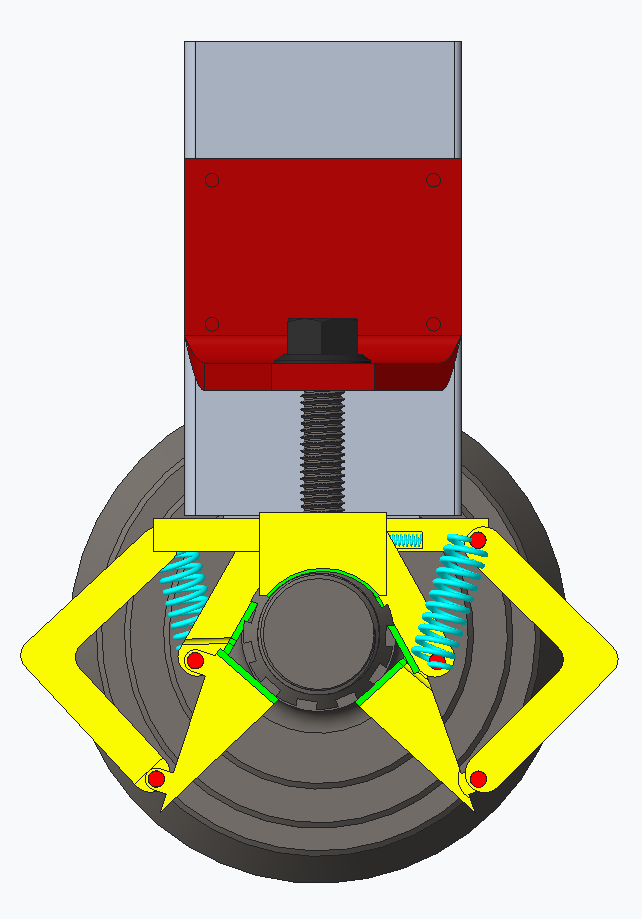
\includegraphics[width=\textwidth]{Immagini/tennis.png}
		\caption*{Test end:\\ the rubber ensures enough pressure on the component to guarantee better pick up}
	\end{minipage}
\end{figure}

\subsection*{Possible future adjustments for Manufacturing}
The following are possible future design improvements to reduce costs and increase ease of manufacturing:
\begin{itemize}
	\item Modify and make the links in sheet metal rather than steel as in the current version.
	\item Perform cuts to further reduce material at various points of the design, such as in the lateral supports.
	\item Add laser cuts also in the bases of the two rotating claws to facilitate the assembly of the part.
	\item Add a metal notch inside the rubber of the claw tips to improve the stability and firmness of the grip.
\end{itemize}